\documentclass[conference]{IEEEtran}
\IEEEoverridecommandlockouts

\usepackage{cite}
\usepackage{amsmath,amssymb,amsfonts}
\usepackage{algorithmic}
\usepackage{graphicx}
\usepackage{textcomp}
\usepackage{xcolor}

\begin{document}

\title{Quantifying Gentrification Technical Report}

\author{\IEEEauthorblockN{Amy Boncelet}
\IEEEauthorblockA{\textit{Jacobs Technion-Cornell Institute} \\
\textit{Cornell Tech}\\
New York City, United States of America \\
ajb347@cornell.edu}
\and
\IEEEauthorblockN{Matthew Shen}
\IEEEauthorblockA{\textit{Jacobs Technion-Cornell Institute} \\
\textit{Cornell Tech}\\
New York City, United States of America \\
mds377@cornell.edu}
\and
\IEEEauthorblockN{Thomas Wallace}
\IEEEauthorblockA{\textit{Jacobs Technion-Cornell Institute} \\
\textit{Cornell Tech}\\
New York City, United States of America \\
tw526@cornell.edu}
}

\maketitle

\begin{abstract}
The following document is a technical write-up on how our team decided to quantify gentrification in New York City. This project was done as part of INFO 5430: Urban Data at Cornell Tech. 
\end{abstract}

\begin{IEEEkeywords}
Urban Technology, Urban Data, Data Science, Information Systems
\end{IEEEkeywords}

\section{Introduction}
The project we conducted had two phases. In the first phase we developed a methodology to quantitatively determine whether a neighborhood had gentrified over a certain period of time. The second part of the project was to apply this methodology to New York City between 2011 and 2019.

\section{Analysis}

\subsection{How we defined gentrification}
In order to define gentrification we looked at six different metrics and observed how they changed over time. An increase in any of these metrics would mean an increase or decrease in gentrification, a summary of our hypothesis can be seen in Table~\ref{gen_metrics}.

\begin{table}[htbp]
\caption{Gentrification Metrics}
\begin{center}
\begin{tabular}{cc}
\hline\hline
\textbf{An increase in this metric =} & \textbf{An increase in this metric =} \\
\textbf{Increase Gentrification} & \textbf{Decrease Gentrification} \\
\hline
\% White Population* & Median Age                                   \\
Median Income        & \% Foreign Born(Non-US Citizen)*              \\
\% Bachelor's Degree* & \\
\% Median Rent &\\
\hline\hline
\multicolumn{2}{l}{Per Capita Calculation Required*}
\end{tabular}
\label{gen_metrics}
\end{center}
\end{table}

These metrics were selected based on \cite{b1}, \cite{b2}, \cite{b3}, and \cite{b4}

\subsection{Project Scope}
Data was collected on the different metrics found in Table~\ref{gen_metrics} through the US Census Bureau. We specifically looked at information between 2011 and 2019. These years were selected because they sat between the decennial censuses in 2010 and 2020. This range of years also allowed us to avoid the 2020 COVID-19 pandemic.

ZCTA5 values were used as the baseline geo-location. This meant that we were comparing demographic information between ZCTA5s. A more granular baseline geo-location would have been census tracts; however, our project looks at long-term changes in areas, and census tracts can change from year to year. ZCTA5 values remain relatively constant which meant that we knew that our geo-location baseline would remain the same.

New York City was selected as the test bed for our analysis.

\subsection{Methodology}

\subsubsection{Year Organization}
The initial data that we received from the United States Census Bureau was collected from four different surveys. These different surveys can be seen in Table~\ref{surveys}.
\begin{table}[htbp]
\caption{US Census Bureau Surveys}
\begin{center}
\begin{tabular}{cc}
\hline\hline
\textbf{Survey Code} & \textbf{Survey Description} \\
\hline
DP05 & ACS Demographic \& Housing Estimates\\
S1901 & Income in the Past 12 Months\\
DP02 & Selected Social Characteristics\\
DP04 & Selected Housing Characteristics\\
\hline\hline
\end{tabular}
\label{surveys}
\end{center}
\end{table}
Each of the surveys also came in separate files for each year. As a result, we had four surveys for each of the nine years. This totaled up to 36 different surveys. These data sets were then merged into each individual year. This meant that we had a consolidated data set with all the survey data each year.

\subsubsection{Column Metadata}
Unfortunately, the column metadata changed for different variables at different points in our analysis. As a result, we had to individually go through each data set and determine how the column names changed with each year. The relevant columns used to subset can be seen in Appendix~\ref{app_A}.

Once all the columns were renamed we subset the data to only include the ZCTA5s, the data in Table~\ref{gen_metrics}, and the total population.

\subsubsection{Cleaning Data Types}
We then found that some of the census data was presented as strings. In order to process the data we had to either convert the data to a float/integer or remove the data.

We also found that the ZCTA5 data was in the format of "ZCTA5 00000". To allow for easier querying we striped the "ZCTA5 " and then changed the five-digit code to an integer.

Another problem we found in the data was that some ZCTA5 values did not have a population. This was due to some new buildings which have independent ZCTA5 values but residences have not moved in. As a result, we decided to remove these values.

The final minor data cleaning measure was to subset the ZCTA5s to only include ones in NYC.

\subsubsection{Interpolating Missing Data}
Once each data set was cleaned and subset we noticed that some data was sporadically missing. In order to fill in this data we interpolated with the nearby ZCTA5 values. This was done because we can make the assumption that ZCTA5 values near each other would have similar statistical values.

\subsubsection{Per Captia Calculations}
The white population, bachelor's degrees, and foreign-born (non-US citizen) data was given to us as raw numbers. We needed to ensure that an increase in these raw values could not be attributed to general trends in the city or changes in population numbers. To mitigate this we took the quotient of these values and the total populations at each ZCTA5s.

\subsubsection{Calculate change over time}
The next step was the look at how our different metrics changed over time. To do this we merged the cleaned data sets from 2011 and 2019 on the ZCTA5s. This would allow us to remove any ZCTA5s that did not exist in both data sets. We then found the difference between 2011 and 2019. Next, we transformed the metrics in Table~\ref{gen_metrics} that decrease gentrification into negative numbers. This ensures that an increase in those values results in a lower gentrification score.

\subsubsection{Normalize data}
We finally normalized the data with Equation~\ref{norm}.
\begin{equation}
\frac{x-\mu}{\sigma}\label{norm}
\end{equation}
In Equation~\ref{norm} $x$ is the value we are changing, $\mu$ is the mean of the series that data set, and $\sigma$ is the standard deviation of the series that data set. This normalization ensured that the magnitude of the values did not effect the gentrification metric.

\subsubsection{Creating the Gentrification Metric}
Now that our data is normalized we can create our gentrification metric by adding all the values in Table~\ref{gen_metrics} for each ZCTA5.

\section{Results}
The gentrification metric was then plotted with respect to each neighborhood. This visualization can be seen in Appendix~\ref{app_b}. From our results, we can see that the ZCTA5's that gentrified the most were: 11216, 10005, 10007, 11221, 11237, 11217, 11238, 11222, 11101, 11225. In contrast the ZCTA5's that gentrified the least were: 10002, 11364, 10469, 10075, 11358, 11356, 11355, 11354, 11239, 10069.

\begin{thebibliography}{00}
\bibitem{b1} A. Owens and J. Candipan, ``Racial/Ethnic Transition and Hierarchy Among Ascending Neighborhoods'' \textit{Urban Affairs Review}, vol. 55, no. 6, Apr. 2018. Accessed: Dec. 4, 2022. doi: https://doi.org/ 10.1177/107808741877081. [Online]. Available: https://journals.sagepub.com/doi/10.1177/1078087418770810

\bibitem{b2} M. Cohen and K. L. S. Pettit, "Guide to Measuring Neighborhood Change to Understand and Prevent Displacement," \textit{National Neighborhood Indicators Partnership(NNIP)}, Boston, MA, 2016. Accessed Dec. 4, 2022. [Online]. Available: https://www.urban.org/sites/default/files/publication/100135/guide\_to\_ measuring\_neighborhood\_change\_to\_understand\_and\_prevent\_ displacement.pdf

\bibitem{b3} T. Buffel and C. Phillipson, “Ageing in a Gentrifying Neighbourhood: Experiences of Community Change in Later Life,” \textit{Sociology}, vol. 53, no. 6, Apr. 2019. Accessed: Dec. 4, 2022. doi: https://doi.org/10.1177/0038038519836848. [Online]. Available: https://journals.sagepub.com/doi/full/10.1177/0038038519836848

\bibitem{b4} J. Hwang, “Immigration is an important dimension in how we understand gentrification across US cities,” \textit{London School of Economics}, Oct. 2015. Accessed: Dec. 4, 2015. [Online]. Available: https://blogs.lse.ac.uk/usappblog/2015/10/21/immigration-is-an-important-dimension-in-how-we-understand-gentrification-across-us-cities/ 


\end{thebibliography}

\clearpage
\appendix[Column Names Over Time]\label{app_A}
\begin{table}[htbp]
\caption{Bachelor's Degree}
\begin{center}
\begin{tabular}{cc}
\hline\hline
\textbf{Year} & \textbf{Code} \\
\hline
2011 & DP02\_0064E \\
2012 &  \\
2013 &  \\
2014 &  \\
2015 &  \\
2016 &  \\
2017 &  \\
2018 &  \\
\hline
2019 & DP02\_0065E \\
\hline\hline
\end{tabular}
\end{center}
\end{table}
\begin{table}[htbp]
\caption{Foreign born, not a US Citizen}
\begin{center}
\begin{tabular}{cc}
\hline\hline
\textbf{Year} & \textbf{Code} \\
\hline
2011 & DP02\_0095E \\
2012 & \\
2013 & \\
2014 & \\
2015 & \\
2016 & \\
2017 & \\
2018 & \\
\hline
2019 & DP02\_0096E \\
\hline\hline
\end{tabular}
\end{center}
\end{table}
\begin{table}[htbp]
\caption{Median Income}
\begin{center}
\begin{tabular}{cc}
\hline\hline
\textbf{Year} & \textbf{Code} \\
\hline
2011 & S1901\_C01\_012E \\
2012 & \\
2013 & \\
2014 & \\
2015 & \\
2016 & \\
2017 & \\
2018 & \\
2019 & \\
\hline\hline
\end{tabular}
\end{center}
\end{table}
\begin{table}[htbp]
\caption{White Non-hispanic}
\begin{center}
\begin{tabular}{cc}
\hline\hline
\textbf{Year} & \textbf{Code} \\
\hline
2011 & DP05\_0072E \\
2012 & \\
2013 & \\
2014 & \\
2015 & \\
2016 & \\
\hline
2017 & DP05\_0077E\\
2018 & \\
2019 & \\
\hline\hline
\end{tabular}
\end{center}
\end{table}
\begin{table}[htbp]
\caption{Median Age}
\begin{center}
\begin{tabular}{cc}
\hline\hline
\textbf{Year} & \textbf{Code} \\
\hline
2011 & DP05\_0017E \\
2012 & \\
2013 & \\
2014 & \\
2015 & \\
2016 & \\
\hline
2017 & DP05\_0018E\\
2018 & \\
2019 & \\
\hline\hline
\end{tabular}
\end{center}
\end{table}
\begin{table}[htbp]
\caption{Rent - Gross rent median price}
\begin{center}
\begin{tabular}{cc}
\hline\hline
\textbf{Year} & \textbf{Code} \\
\hline
2011 & DP04\_0132E \\
2012 & \\
2013 & \\
2014 & \\
\hline
2015 & DP04\_0134E\\
2016 & \\
2017 & \\
2018 & \\
2019 & \\
\hline\hline
\end{tabular}
\end{center}
\end{table}

\clearpage
\appendix[Gentrification Map]\label{app_b}
\begin{figure}[htbp]
\centerline{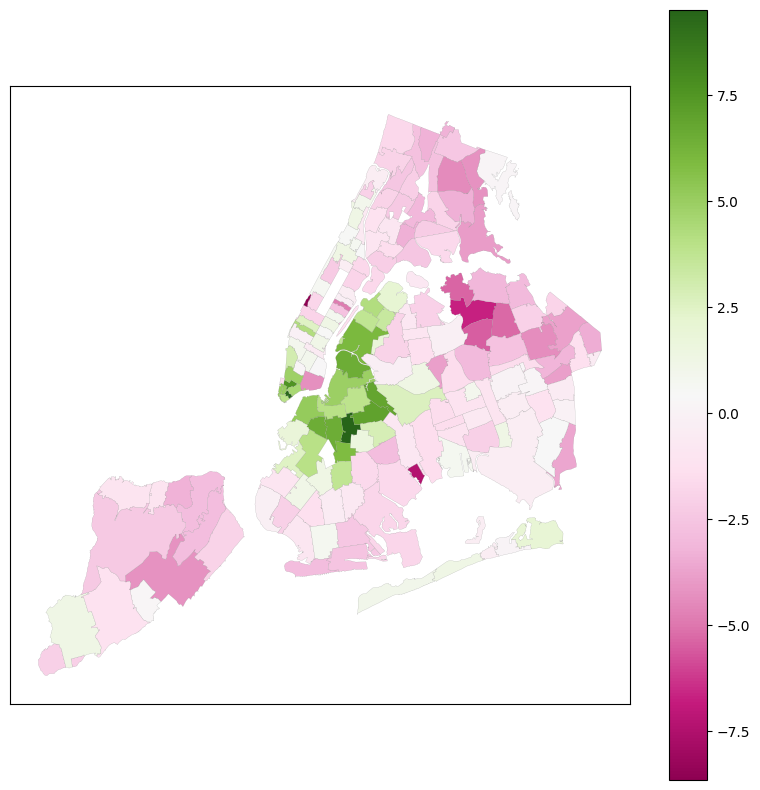
\includegraphics[width=0.45\textwidth]{images/gen_map.png}}
\end{figure}

\end{document}
